\section{Theory}
\label{sec:theory}

This section is devoted to laying out a more formal description of the
theory presented in Section~\ref{sec:intro}. While the particles and
their properties tabulated in Figure~\ref{fig:sm} summarize the important
players in the study of elementary particles, an understanding of the
mathematical ideas behind the Standard Model are essential in grasping
the importance of this measurement. Section~\ref{subsec:qed} gives a brief
introduction to Gauge Theory and Quantum Field Theory through the simplest
theory contained in the Standard Model: Quantum Electrodynamics (QED).
Afterward the Higgs Mechanism is explained in Section~\ref{subsec:higgsmec}
and finally the production processes studied in this measurement are
given in Section~\ref{subsec:prodproc}.


\subsection{Introduction to Gauge Theory and Quantum Field Theory}
\label{subsec:qed}

There are many ways to analyze the dynamics of a particle classically; however,
the one most suited for studying the symmetries of a system is Lagrangian Mechanics.
The study of such a systems begins by defining a Lagrangian function as
\begin{equation}
    L(q, \dot q) = T - U 
\end{equation}
where $T$ and $U$ are the particle's kinetic and potential energy respectively, 
so that the Lagrangian is a function of the particle's coordinates and velocities. 
The mathematics behind the Standard Model is formulated in terms of the Langrian
approach to mechanics; however, a minor detail arises because the Standard Model
describes fields not particles.

The Standard Model is a Quantum Field Theory meaning that it is not interested in
describing particles, which are localized entities, but in describing the
dynamics of fields, which occupy some extended region of space. For example the
electromagnetic field $\mathbf{E}$ is a vector vield that is described 
by three component functions that can change throughout space and time: 
$\mathbf{E}(\phi_i) = (\,\phi_x(x,y,z,t), \phi_y(x,y,z,t), \phi_z(x,y,z,t)\,)$. 
As such the Lagrangians contained in the Standard Model are functions of these
fields and their derivative.

As an introduction to how these mathematical formalism works let's consider the
Lagrangian descibing QED:
\begin{equation}
\mathcal{L} = \frac{-1}{16\pi}\left(\partial^{\mu} A^{\nu} - \partial^{\nu}A^{\mu}\right) = 
\frac{-1}{16\pi} F^{\mu\nu}F_{\mu\nu}.
\end{equation}
were $A^{\mu} = (\phi, \mathbf{A})$ is the electomagnetic potential.

\subsection{The Higgs Mechanism}
\label{subsec:higgsmec}

\subsection{Production Process}
\label{subsec:prodproc}

\begin{figure}[!htbp]
  \begin{center}
  {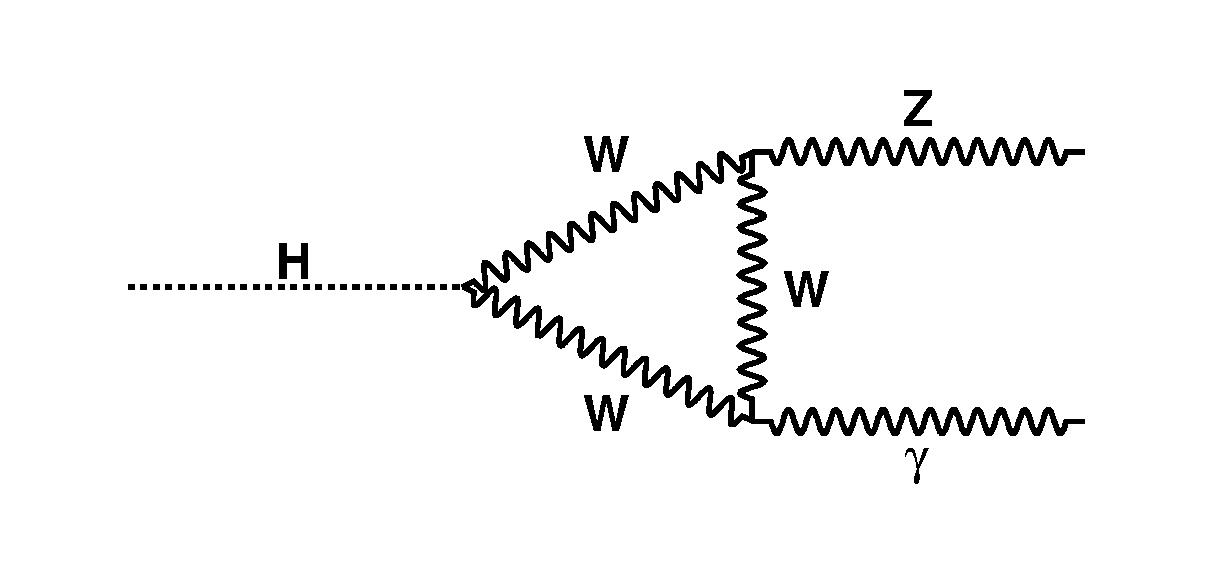
\includegraphics[width=2in]{figures/loop1}}
  {\includegraphics[width=2in]{figures/loop2}}
  {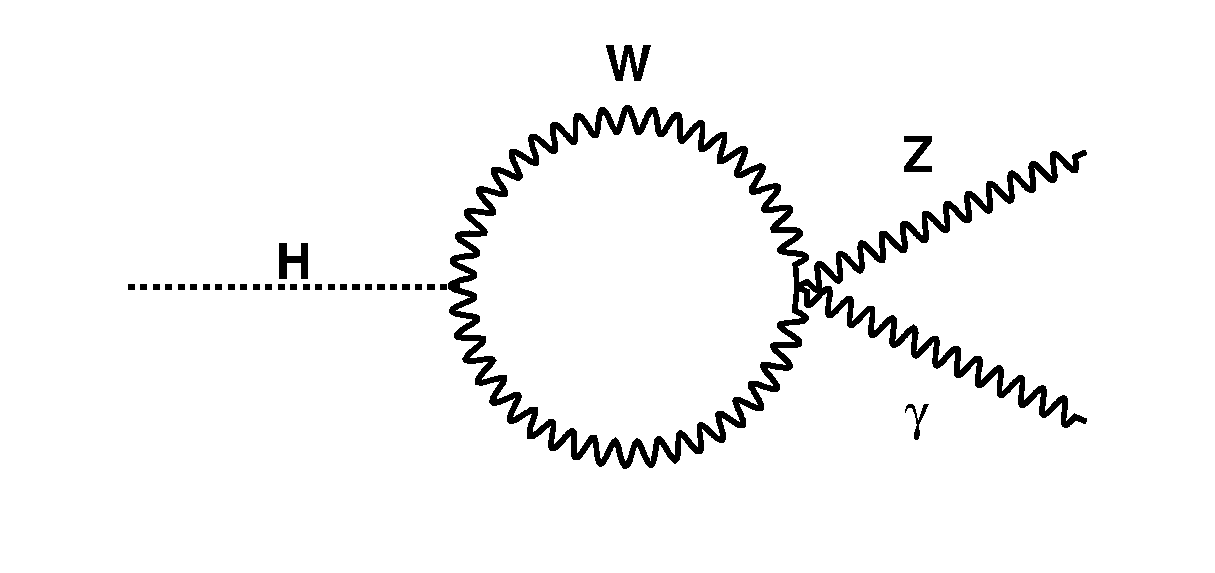
\includegraphics[width=2in]{figures/loop3}}
  \caption{Leading Feynman diagrams for the $H\rightarrow Z\gamma$
    decay in the Standard Model. Note that in the case of the fermion
    loop, top quarks dominate.} 
  \label{fig:feynman}
  \end{center}
\end{figure}

